\documentclass{article} % Tipo de documento

\usepackage[utf8]{inputenc} % Permite el uso de caracteres del Español

\usepackage[T1]{fontenc}

\usepackage{graphicx}

\usepackage{subfig}

% Carátula del Artículo  

\title{Reporte de Actividad 5}

\author{Brenda Leyva Amaya}

\date{6 de Marzo, 2018}
 

\begin{document}

\maketitle % Crea el título


\section{Introducción.}

En la presente actividad se llevó a la práctica la adquisición de una serie de datos y su posterior limpieza. Es importante tener este tipo de práctica pues al manipular grandes cantidades de información no es posible llevar a cabo una modificación de manera manual, linea por linea, aquí entran otro tipo de técnicas más eficientes, desde la automatización de su obtención y transformación de los archivos así como la elección especifica de cierta información necesaria y discriminación de aquella que solo ocasionaría ruidos en el análisis correspondiente.

\section{CAPE y PW.}

\hspace{0.45 cm} - CAPE - Convective available potential energy.

\vspace{0.5 cm}

Su significado en español "Energía potencial conectiva disponible". En meteorología, CAPE es la cantidad de energía un "diferencial" de aire tendría si se levantara una cierta distancia vertical a través de la atmósfera. Es la flotabilidad positiva efectiva de dicho "paquete" de aire y es un indicador de la inestabilidad atmosférica, lo cual le hace muy valioso para predecir climas severos. CAPE es una forma de fluido inestable que se encuentra en atmósferas estratificadas de manera térmica, en las que un fluido más frío cubre a uno más caliente. Cuando una masa de aire es inestable, el elemento de esta masa es desplazado hacia arriba y acelerado por la presión diferencial entre el aire desplazado y el aire del ambiente en las altitudes más altas. Esto usualmente crea nubes de convección debido al incremento en movimiento lo cual puede eventualmente llevar a el desarrollo de tormentas y fenómenos como frentes fríos. 

\vspace{0.5 cm}

- PW - Precipitable water.

\vspace{0.5 cm}

El agua precipitable es la profundidad del agua en una columna de la atmósfera, si toda el agua de esa columna se precipitara como lluvia. Como profundidad está medida en milímetros o pulgadas. Comunmente se abrevia como "TPW" y es igual al total de agua precipitable. 


\section{Limpieza y preparación de datos.}

La limpieza de datos se llevó a cabo con ayuda de la herramienta Emacs, en la cual se pueden eliminar grandes cantidades de información "basura" con comandos simples que actúan rápidamente y nos ayudan a conformar archivos o series de datos con características muy especificas a la actividad que se realizará con ellos posteriormente. 	

\vspace{0.5 cm}

Las primeras acciones de limpieza se referían a la eliminación de ruido, o sea de los datos e información repetitiva que no se utilizaría en la actividad pues solo generarían complicaciones innecesarias a la hora de manipular los datos. 

\vspace{0.5 cm}

A continuación se utilizaron comandos de manera similar a la limpieza pero para generar un formato que llevara a pandas a una lectura fácil y clara y evitar errores en los análisis y la graficación de los datos. 

\section{Análisis de datos.}

A continuación se presentan los resultados del análisis gráfico de la información obtenida para la actividad. El lugar al cual corresponden los datos es la estación meteorológica de Budapest. Esta ciudad es la capital y la ciudad más poblada de Hungría, también es su principal centro industrial. La ciudad tiene un clima húmedo continental, un clima de transición entre el templado cubierto de nieve en Transdanubia y el clima variable de la gran llanura plana y abierta del este, además del clima sub-mediterráneo del sur. 

\vspace{0.5 cm}

La primavera se caracterica por la abundancia de sol y lluvias aisladas. La temperatura comienza a subir en abril, por lo general alcanzando máximas de 25 grados centígrados al final de ese mes. SIn embargo hay zonas donde las heladas continúan incluso en el mes de mayo. En los veranos existen periodos prolongados de calor y temperaturas entre 32 y 35 grados, las cuales se intercambian con breves periodos húmedos con frentes fríos provenientes del oeste cuyas temperaturas están entre 18 y 25 grados. 

\vspace{0.5 cm}

Las temperaturas altas pueden mantenerse por encima de los 20 grados hasta el final de octubre. Las noches más frías y las heladas llegan por primera vez por lo general en la segunda semana de octubre. En noviembre sobreviene la abundante lluvia y en ocasiones nieve y una caída drástica de la temperatura. 

\vspace{0.5 cm}

Los inviernos son variable e impredecibles, los vientos del oeste traen aire templado oceánico el cual dispersa la lluvia o la nieve. Las borrascas que se desplazan desde el mar Mediterráneo pueden traer tormentas de nieve con 20 a 40 cm de caída en un solo día. 

\vspace{0.5 cm}

La primer imagen nos muestra las gráficas de caja correspondientes a las mediciones de 00z y 12z anuales de CAPE.    

\begin{center}%

\begin{figure}%
    \centering
    \subfloat[CAPE-00Z]{{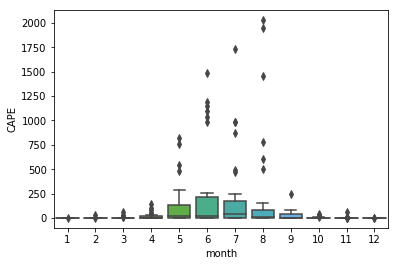
\includegraphics[width=5cm]{00Z-1.png} }}%
    \qquad
    \subfloat[CAPE-12Z]{{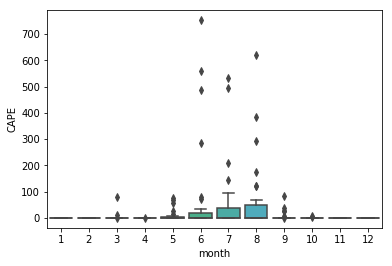
\includegraphics[width=5cm]{12Z-1.png} }}%
    \caption{Gráficos de caja para CAPE en las tomas de 00z y 12z respectivamente.}%
\end{figure}
	
\end{center}%

A continuación se presentan los gráficos de caja para los valores de agua precipitable en la figura 2. 

\begin{center}%

\begin{figure}%
    \centering
    \subfloat[PW-00Z]{{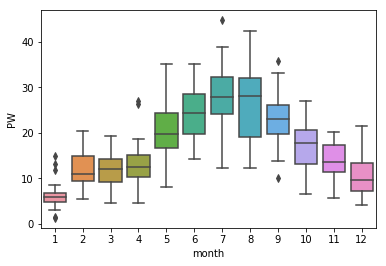
\includegraphics[width=5cm]{00Z-2.png} }}%
    \qquad
    \subfloat[PW-12Z]{{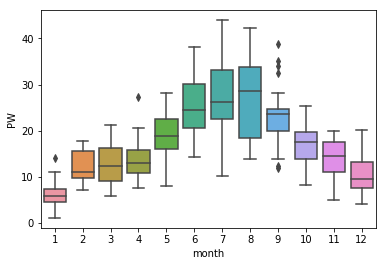
\includegraphics[width=5cm]{12Z-2.png} }}%
    \caption{Gráficos de caja para PW en las tomas de 00z y 12z respectivamente.}%
\end{figure}
	
\end{center}%

La figura 3 relaciona los valores de CAPE y PW para tratar de encontrar una relación entre ellas o indicar si no existe alguna. 

\begin{center}%

\begin{figure}%
    \centering
    \subfloat[CAPE VS PW - 00Z]{{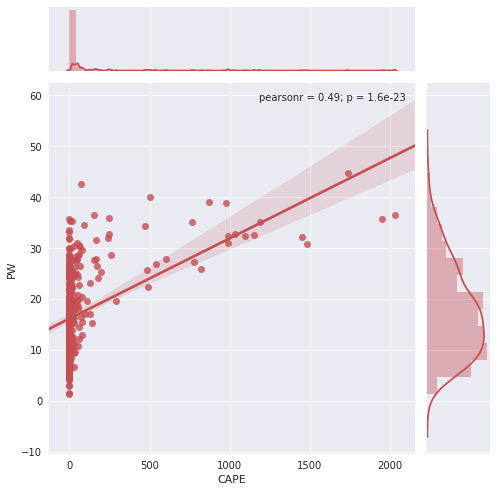
\includegraphics[width=5cm]{00Z-3.png} }}%
    \qquad
    \subfloat[CAPE VS PW - 12Z]{{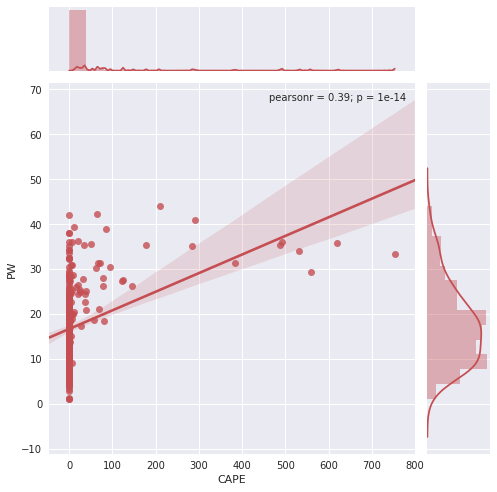
\includegraphics[width=5cm]{12Z-3.png} }}%
    \caption{Relación entre CAPE y PW para las dos series de datos.}%
\end{figure}
	
\end{center}%

Finalmente se observa en la figura 4 

\begin{center}%

\begin{figure}%
    \centering
    \subfloat[00Z-4]{{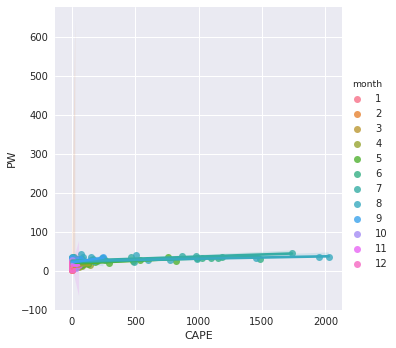
\includegraphics[width=5cm]{00Z-4.png} }}%
    \qquad
    \subfloat[12Z-4]{{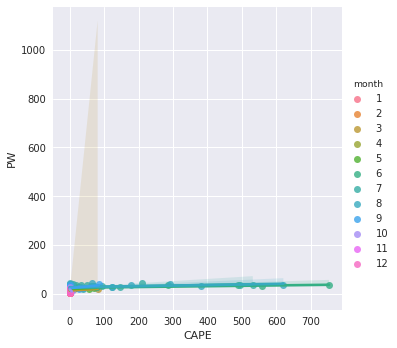
\includegraphics[width=5cm]{12Z-4.png} }}%
    \caption{Comparativo 4.}%
\end{figure}
	
\end{center}%

\section{Resultados.}

Para cada uno de los análisis que se llevaron a cabo se pueden encontrar valores "extraordinarios" sesgos que se encuentran totalmente fuera de las aparentes distribuciones o tendencias, pero para efectos de comprender un poco mejor este fenómeno es que se han incluido algunos datos y características principales del clima de la región.

\vspace{0.5 cm}

En base a esto podemos decir que el comportamiento gráfico es el esperado pues coincide con las características del lugar ya que es una región de climas extremosos en la cual en una temporada de verano pueden existir cortos periodos de frentes fríos y precipitaciones así como elevaciones drásticas de la temperatura por encima de los 30 grados. 


\section{Conclusiones.}

La actividad se ha llevado a cabo con satisfacción en el tiempo disponible, sin embargo se han encontrado retos en lo que respecta a la interpretación correcta de datos y a la manipulación de imágenes y su colocación estética en la herramienta LaTex.
	
\vspace{0.5 cm}

Se espera en el transcurso de la clase adquirir más y  mejores habilidades que permitan superar estos obstáculos y permitan la creación de actividades y reportes de estas con una mejor calidad y presentación más adecuada y amigable con el lector de las mismas. 

\vspace{0.5 cm}

Por otro lado fué interesante observar que el comportamiento gráfico que se obtuvo tiene una relación directa con el teórico y esperado. 


\section{Bibliografía y fuentes.}

Convective available potential energy. (2018, February 28). Retrieved March 05, 2018, from https://en.wikipedia.org/wiki/Convective\_available\_potential\_energy 	
   
\vspace{0.5 cm}

Precipitable water. (2018, February 17). Retrieved March 05, 2018, from https://en.wikipedia.org/wiki/Precipitable\_water 

\vspace{0.5 cm}

Budapest. (2018, February 15). Retrieved March 06, 2018, from https://es.wikipedia.org/wiki/Budapest\#Clima


\section*{Apéndice}

\hspace{0.45 cm} ¿Cómo se te hizo esta actividad? ¿Compleja, Difícil, Sencilla?

\vspace{0.5 cm}

**La actividad en sí fué sencilla, sin embargo se tomó un tiempo en comprender lo que se solicitaba en un inicio. Una vez comprendidas las instrucciones la actividad fluyó de manera positiva y más rápida de lo esperado. 

\vspace{0.5 cm}

¿Qué te llamó más la atención?

\vspace{0.5 cm}

**Me gustó tener la capacidad de manipular archivos de distintas maneras y para distintos fines desde terminal. 

\vspace{0.5 cm}

¿Qué parte fue la que menos te interesó hacer?

\vspace{0.5 cm}

**La limpieza por medio de comandos de las grandes cantidades de datos, a pesar de ser mucho mejor y mas viable que de manera manual, fue la actividad que más tiempo llevó realizar y la cual era muy mecanizada y menos "divertida" o interesante de la sesión.

\vspace{0.5 cm}

¿Cómo mejorarías esta actividad? ¿Qué le faltó? ¿Qué sobró?

\vspace{0.5 cm}

**Creo que los cambios que podría realizar entran en el aspecto personal, considero que podría haber realizado la limpieza de mejor manera o quizá más automatizada si tuviera mejor conocimiento del uso de scripts. 

\vspace{0.5 cm}

¿Hasta este punto, que te parece el uso de Jupyter para programar en Python? 

\vspace{0.5 cm}

**Jupyter es extremadamente "user friendly" amigable con el usuario y esto lleva a una mejor experiencia de aprendizaje dle nuevo lenguaje de programación.

\vspace{0.5 cm}

\end{document}